% \section{Atividades}
%
% Neste módulo, foram realizadas atividades práticas relacionadas à
% virtualização, configuração de firmware, criptografia de armazenamento e uso de
% containers no ambiente Kali Linux.
%
% Inicialmente foram executados procedimentos de exploração de um hypervisor Tipo
% 2 por meio do Oracle VM VirtualBox no Kali Linux, permitindo analisar suas
% configurações internas, opções de idioma e parâmetros de interface. Em seguida,
% foi criada uma máquina virtual baseada na imagem Debian Netinst, demonstrando o
% processo de configuração de recursos básicos para virtualização em ambiente
% controlado.
%
% Posteriormente, foi realizada a exploração de uma interface UEFI/BIOS em modo
% simulado, utilizando recurso disponibilizado pela Lenovo, permitindo observar
% parâmetros de inicialização, segurança e ordem de boot em firmware moderno.
%
% Na sequência, foi implementada criptografia de disco em partição dedicada
% utilizando LUKS (\textit{Linux Unified Key Setup}), incluindo criação de
% partição, formatação criptográfica, desbloqueio e montagem em diretório do
% sistema de arquivos, demonstrando fundamentos de \textit{Full Disk Encryption}
% (FDE).
%
% Por fim, foram executadas atividades envolvendo o uso de containers Docker no
% Kali Linux, incluindo obtenção de imagem Ubuntu, execução de container
% interativo, monitoramento de processos e encerramento controlado do ambiente,
% permitindo compreender conceitos introdutórios de conteinerização.
%
% \newpage
%
\question[Atividade 10.6]{Exploração do VirtualBox no Kali Linux}

\begin{figure}[H]
  \centering
  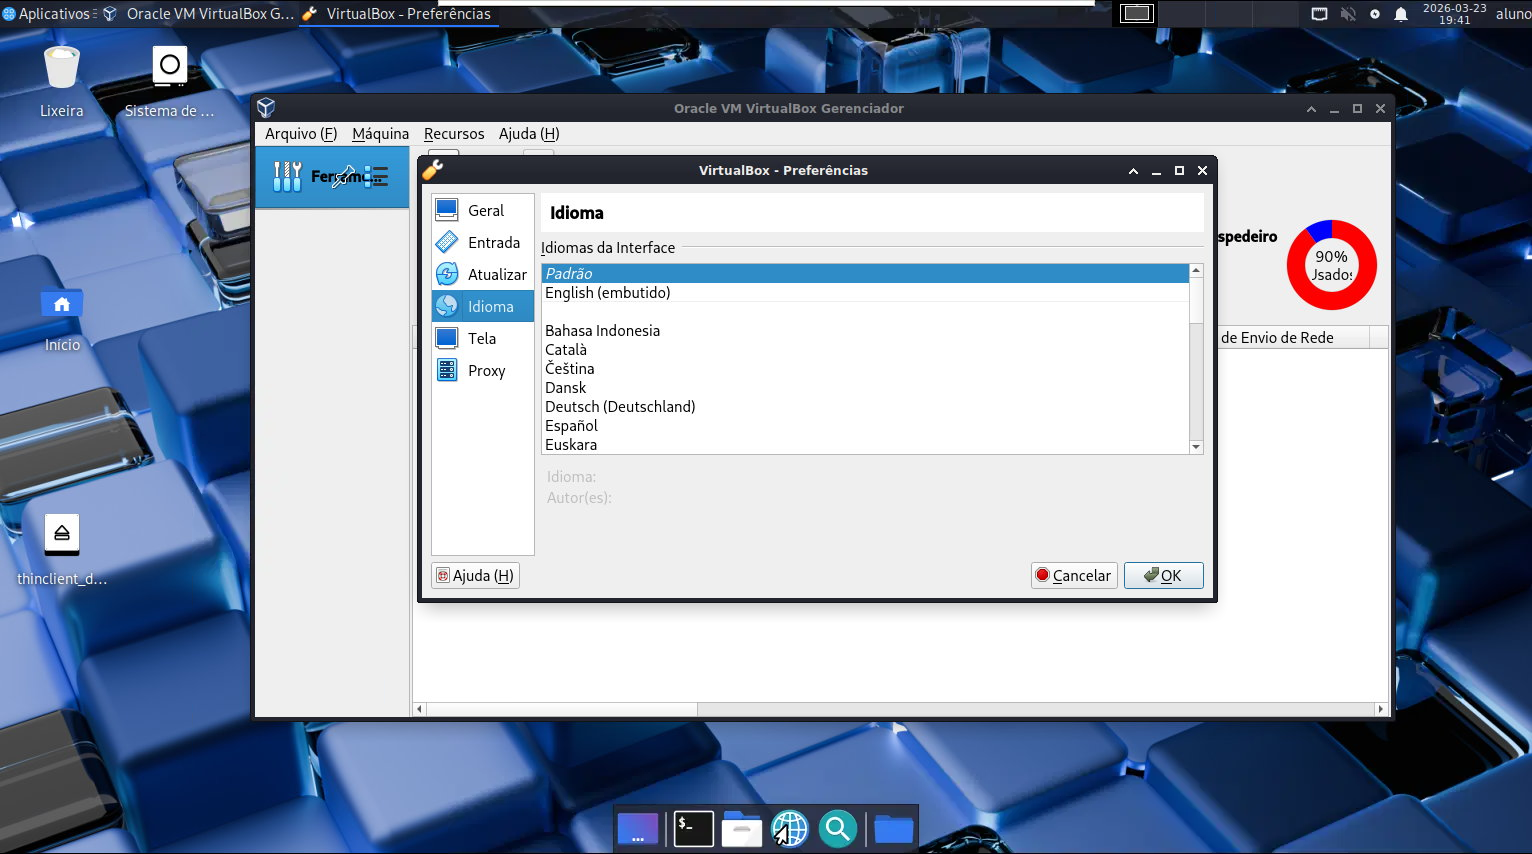
\includegraphics[width=0.99\textwidth]{./fig/fig10.6.png}
  \caption{Visualização da aba de idiomas nas preferências do VirtualBox}
  \label{fig:fig10.6}
\end{figure}

\newpage

\question[Atividade 10.7]{Criação de Máquina Virtual DebianNetinst}

\begin{figure}[H]
  \centering
  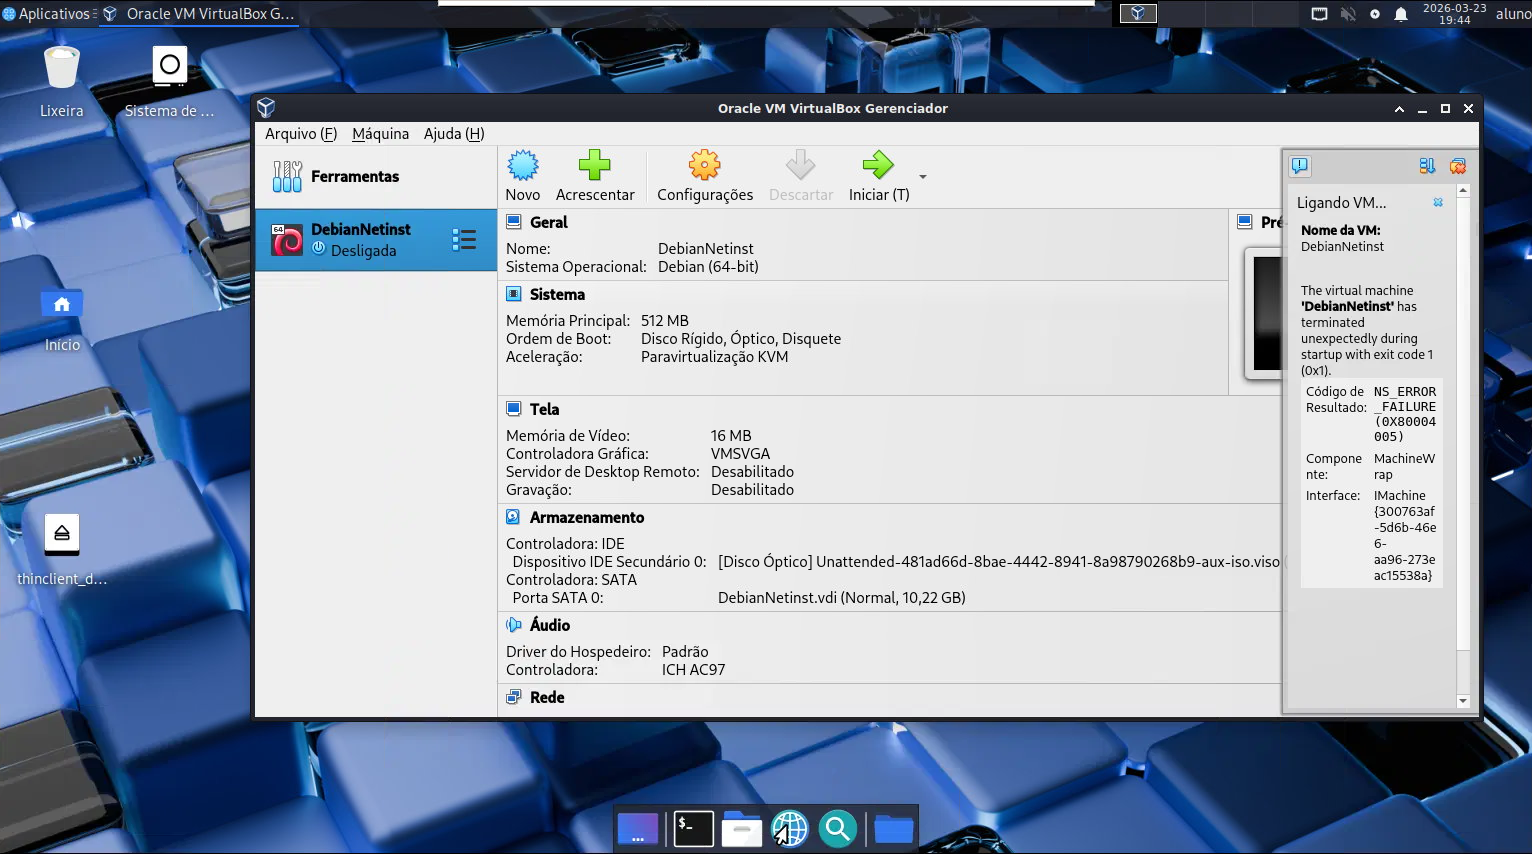
\includegraphics[width=0.99\textwidth]{./fig/fig10.7.png}
  \caption{Máquina virtual DebianNetinst criada e listada no VirtualBox}
  \label{fig:fig10.7}
\end{figure}

\newpage

\question[Atividade 10.8]{Exploração de BIOS/UEFI em Simulador Lenovo}

\begin{figure}[H]
  \centering
  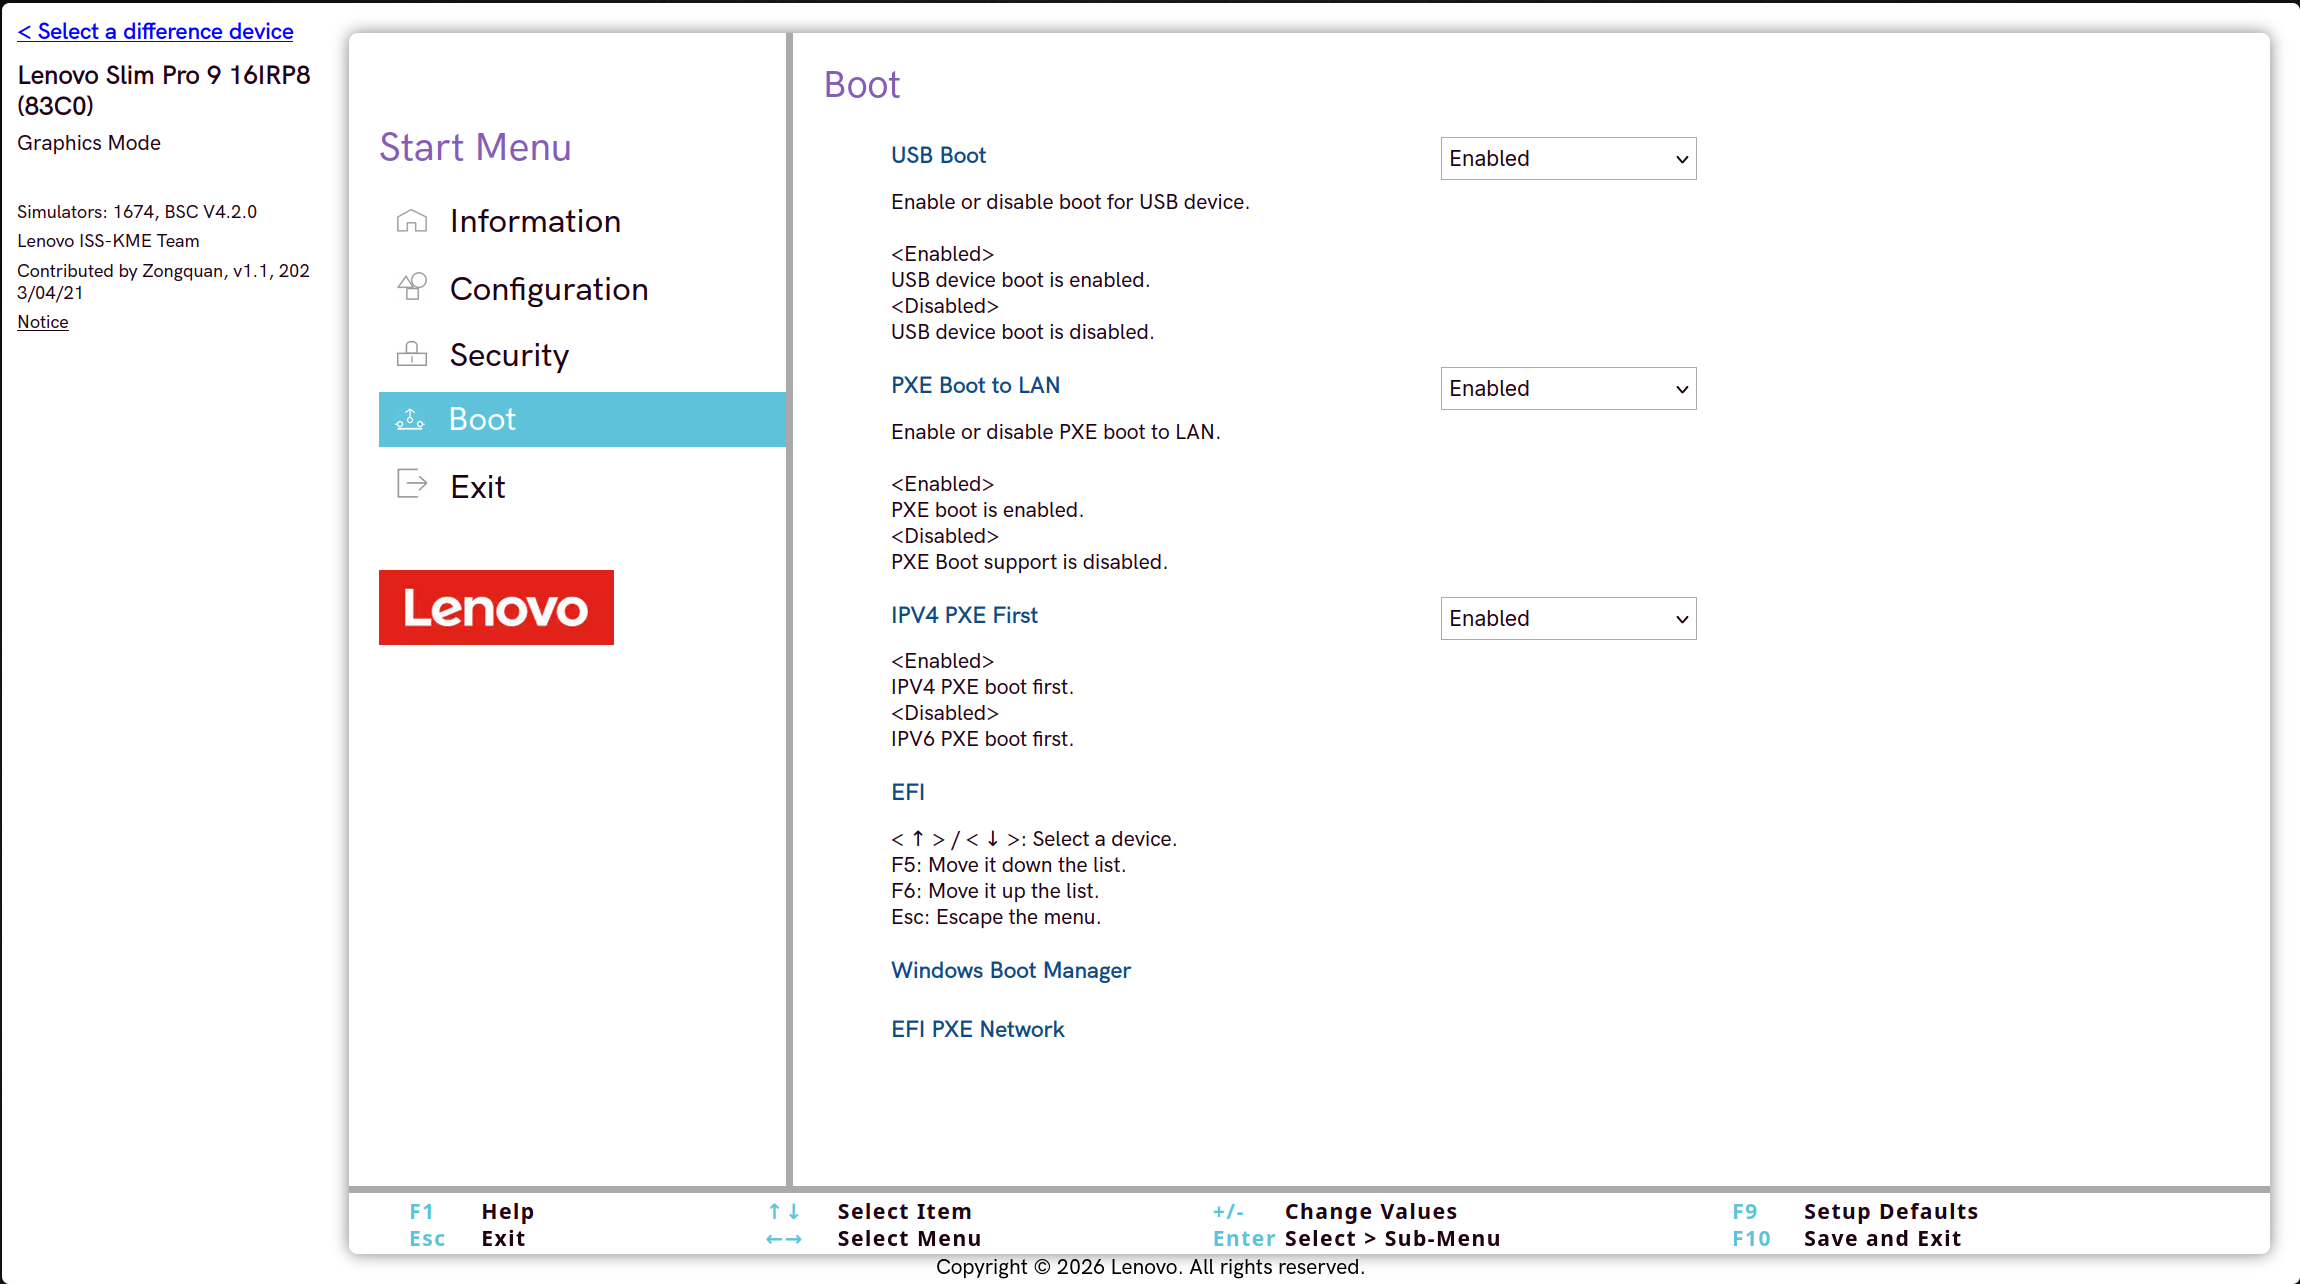
\includegraphics[width=0.99\textwidth]{./fig/fig10.8.png}
  \caption{Tela de configuração de boot na BIOS simulada da Lenovo}
  \label{fig:fig10.8}
\end{figure}

\newpage

\question[Atividade 10.9]{Implementação de Full Disk Encryption com LUKS}

\begin{figure}[H]
  \centering
  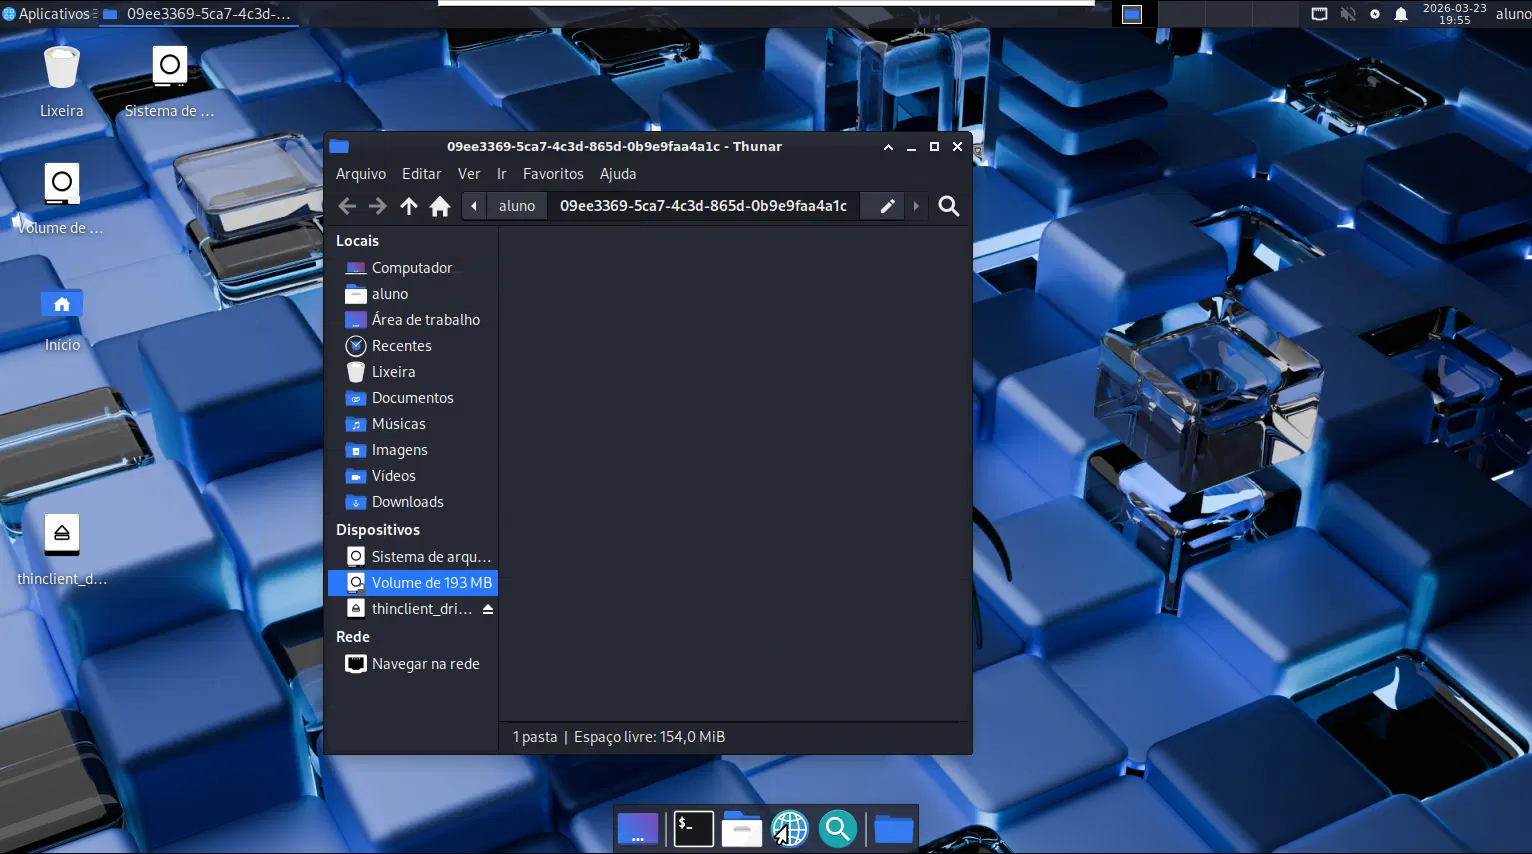
\includegraphics[width=0.99\textwidth]{./fig/fig10.9.png}
  \caption{Acesso ao volume criptografado montado no gerenciador de arquivos Thunar}
  \label{fig:fig10.9}
\end{figure}

\newpage

\question[Atividade 10.10]{Execução de Container Ubuntu com Docker}

\begin{figure}[H]
  \centering
  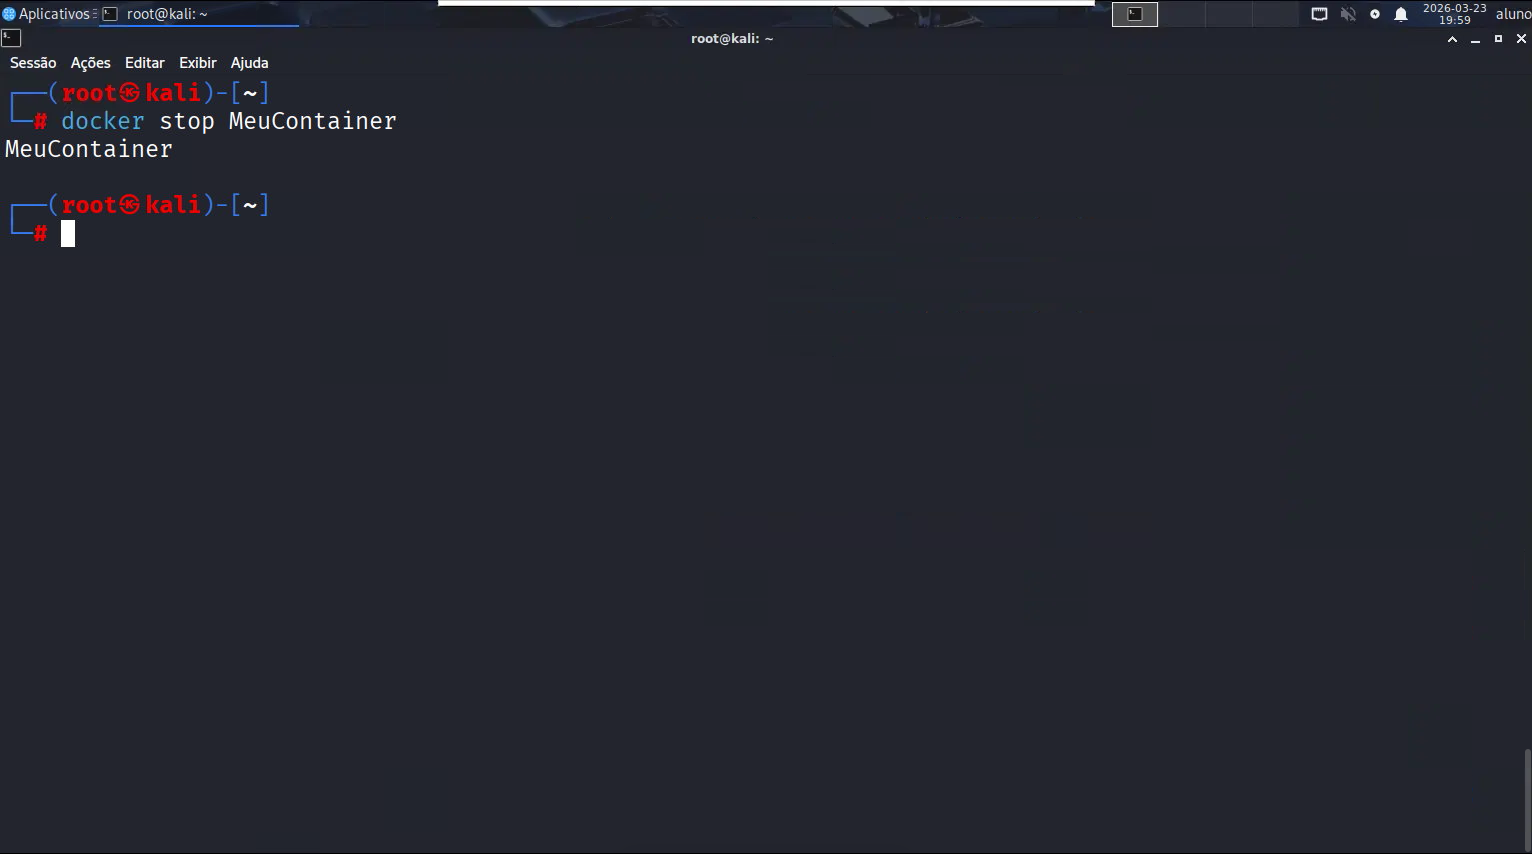
\includegraphics[width=0.99\textwidth]{./fig/fig10.10.png}
  \caption{Parada do container Ubuntu utilizando o comando docker stop}
  \label{fig:fig10.10}
\end{figure}
